\documentclass[a4paper, 14pt, fleqn]{extarticle}
\usepackage[russian]{babel}
\usepackage{fefutitle}
\usepackage[justification=centering]{caption}
\usepackage{float}

\author {
	Группа Б9120-01.03.02миопд\\
	Агличеев Александр
}
\title {
	Отчёт по лабораторной работе №2
}
\date {
	\today
}

\begin{document}
	\maketitle
	\pagebreak
	\parskip = 5pt

	\section{Решение краевой задачи}
		\subsection{Постановка задачи}
			\noindent Необходимо краевую задачу методом Галеркина для дифференциального
			уравнения второго порядка ($x \in [0;1]$):
			\begin{equation*}
				\begin{cases}
					u'' - (1+x)u' - u = \dfrac{2}{(x+1)^3},
					\\
					u(0) = 1,
					u(1) = 0.5. 
				\end{cases}
			\end{equation*}
	
		\subsection{Решение}
			
			\subsubsection{Метод Галеркина}
			
				Решение будем искать в виде 
				\[ u(x) = \phi_0(x) + \sum_{i=1}^{2}C_i \phi_i(x) \]
				, где $\phi_0(x)$ удовлетворяет каждому из краевых условий, функции $\phi_1(x)$ и $\phi_2(x)$ -- линейно независимые, непрерные функции вместе со своими вторыми производными до второго порядка, удовлетворяющие однородным граничным условиям.
				
				В качестве базисным функций выберем полиномы:
				
				\begin{equation*}
					\begin{cases}
						\phi_0(x) = ax+b, \\
						\phi_1(x) = ax^2 + bx + c, \\
						\phi_2(x) = ax^3 + bx^2 + cx + d.
					\end{cases}
				\end{equation*}
				
				Тогда:
				\begin{equation*}
					\begin{cases}
						\phi_0(x) = 1 - \dfrac{1}{2}x , \\
						\phi_1(x) = 0, \\
						\phi_2(x) = x^2-x.
					\end{cases}
				\end{equation*}
			
				Тогда численное решение: 
				\[ u(x) = 1 - \dfrac{1}{2}x + C_2(x^2-x) \]
				\[u'(x) = -\dfrac{1}{2} + C_2(2x-1) \]
				\[u''(x) = 2C_2\]
				
				Подставим $u''(x)$, $u'(x)$, $u(x)$ в дифференциальное уравнение
				\[ R(x, C_1, C_2) = C_2(-3x^2+3) + x - \dfrac{1}{2} - \dfrac{2}{(x+1)^3} \]
				Условия ортогональности функции $R(x, C_1, C_2	)$ к функциям $\phi_1(x)$, 
				$\phi_2(x)$ приводят к системе:
				\[ \int_{0}^{1} \phi_1(x)R(x, C_1, C_2)dx = 0, 
				\int_{0}^{1} \phi_2(x)R(x, C_1, C_2)dx = 0 \]
				Подставляя вместо $R(x, C_1, C_2)$ и $\phi_i(x)$ нужные значения, после
				соответсвующего интегрирования и решения СЛАУ, найдём $C_1$ и $C_2$.
				\begin{equation*}
					\begin{cases}
						C_1 = 0 , \\
						C_2 = 0.325.
					\end{cases}
				\end{equation*}
				В итоге решение имеет вид:
				\[ u(x) = 1 - \dfrac{x}{2} + 0.325(x^2-x) \]
				
			\subsection{Сравнение между точным и приближенным значением}
				 Найдем разницу между точным и приближенным решением на отрезке [0, 1] с шагом
				 $h = 0.1$. $y_i*$ - точное решение, $y_i$ - приближенное.
				 
				 Точное решение $u(x) = \dfrac{1}{x+1} $
				 
 				\begin{figure}[h]
				 	\centering
				 	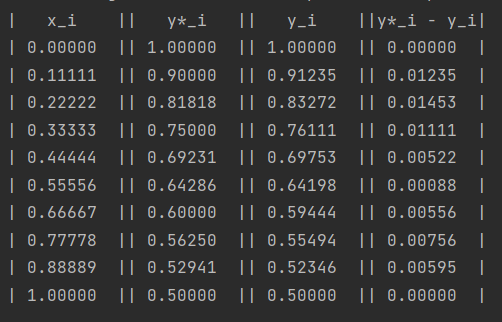
\includegraphics[width = 0.7\linewidth]{table.png}
				\end{figure}
				\pagebreak
				\begin{figure}[h]
					\centering
					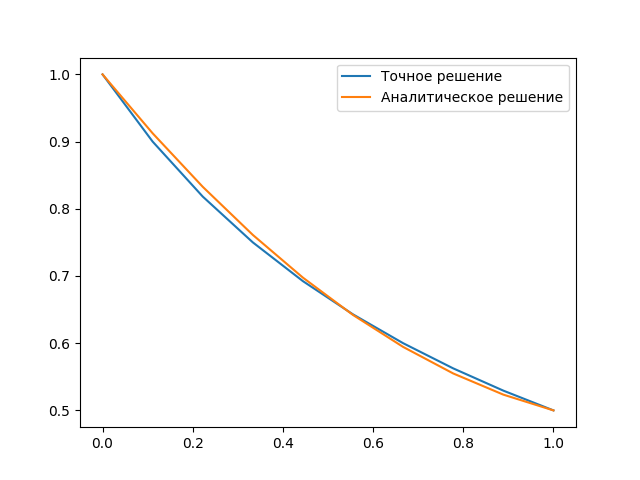
\includegraphics[width = 0.9\linewidth]{plot.png}
				\end{figure}
\end{document}	